\chapter{(Financial) yield - upscaling}
Performances of Aquifer Storage and Recovery systems (ASR-systems) are so far expressed in water volumes. The volumetric results are desirable, but it is hard to get a good picture of it. Simplistic transformations make it possible to express the obtained volumes in (financial) yields. Moreover, the transformation houses the transition from volumes of water to actual sizes of agricultural fields. This part of research offers a glimpse in system (financial) feasibility and potential of system spatial multiplication. \\

First, an explanation on applied theories in transition from water volumes to agricultural field-sizes and financial yields (Section \ref{section:Theory_yields}). Subsequently the previously obtained water volumes are exposed to the transformation (Section \ref{section:Data_processing}). This part of research ends with a conclusive remark on ASR-system yields and posibilities in spatial multiplication (Section \ref{section:Yields_conclusions}). 

\section{Theory: ASR-system - (financial) yield}
\label{section:Theory_yields}

\subsection{Crops: financial yield}
Some crops need more water than others. Some crops thrive better in northern Ghana climate than other. Some crops are financially more beneficial than others. And so, many more elements are decisive in the process of crop type determination. This research is not about crop type decisions. Keeping northern Ghana applicability in mind a selection of crops is made. The crops (mentioned below) are purely included in the study to gain knowledge on hand-on possibilities in the agricultural use of ASR-systems. \\

\textbf{Crops of interest}
\begin{itemize}
\item{Groundnut} \\
Groundnut is an above average profitable crop grown in Ghana. Production is often the responsibility of small holder farmers in the North. Almost the complete Ghana groundnut production originates here \citep{Ghana-made2018}. Growth season length is dependent on the varieties (sequential or alternately). In general harvesting can take place after a period of 90 to 140 days. It is assumed two consecutive growth period fit the (243 days) modelled dry season. For a proper single season production (rain-fed) crops require a water footprint of about 500 to 700 mm. The latter is adapted as normative in this research. Crop yields diverge strongly. Good rain-fed crops can produce average yields of 2-3 ton/ha unshelled nuts. By the introduction of irrigation these values even reach 3.5-4.5 ton/ha \citep{FoodandAgriculturalOrganisationoftheUnitedNationsFAO2018a}. For the subsequent parts of research 2016 Ghana average is used. An agricultural yield of 1.25 ton/ha unshelled groundnut is accounted \citep{FoodandAgriculturalOrganisationoftheUnitedNationsFAO2018}. Financial yields are highly fluctuating over time. Market forces are dominant in actual returns. The march 2018 Ghana average unshelled groundnut wholesale price is set at a value ranging from 247.50 to 282.50 GHS for a 82 kg bag \citep{ModernGhana2018}. For the purposes of this research the highest average value is applied and interpreted as the unshelled groundnut price: 3.445 GHS/kg. 

\item{Other options} \\
* if desirable the same can be done for crops as: Maize, chilli pepper, onion, cucumber, tomatoes, carrots. 
\end{itemize}

As visible assumptions are abundant in size and quantity. Obtained (financial) yields should solely be interpreted as indicative. In other words, "All rights reserved". \\
 
\textbf{Irrigation efficiency} \\
Dry season agriculture is purely dependent on water supply by irrigation. Different types of irrigation are suitable in northern Ghana. One can think of border strip/furrow irrigation; simplistic but inefficient. Higher degrees of efficiency can be achieved by the use of sprinkler irrigation. In the particular case of ASR-system use, minimum water losses are pursued. High efficiency drip irrigation is applied. Systems are standard paired with facilities as poly-tank(s), pipes and drip hoses. Distances between extraction and irrigation are small, resulting in limited losses. However, water losses are present due to pipe connections and potential evaporation. All-encompassing a irrigation system efficiency of 0.8 (-) is considered. 80\% of all water withdrawn is assumed as net usable for crop growth. Note, this efficiency number also accounts for the in practice required schedule in irrigation water amounts. Over the growth season required water volumes are assumed to be daily equal \ref{VandeGiesen2013}. \\

\textbf{Cover area (crop specific)} \\
Water volumes obtained in previous research sections are basic input for the determination of agricultural field sizes. Net withdrawn (dry season) total volumes are divided by the crop specific water footprint. The areal outcome is halved to correct for the double (consecutive) growth periods in a single dry season.   

\begin{equation}
 A = \frac{V_{out,tot} * Water footprint_{crop}}{2 * \eta_{irrigation}} 
\label{eq:A}
\end{equation}

Where, A (m$^2$) is the agricultural field area, $V_{out,tot}$ (m$^3$) is the dry season total volume discharged, $\eta_{irrigation}$ (-) is the irrigation efficiency and $Wfp_{crop}$ is the crop specific water footprint. \\

The extraction of water leaves marks on nature. Pump operation causes a groundwater cone of depression. Close range (and most definitely in-well) drawdown is significant. At an increased radial distance impact losses magnitude. For system spatial multiplication it is of interest to define a maximum circular area in-which groundwater is affected. The groundwater cone of influence (G) is defined as the area corresponding with the maximum radius from well at which the groundwater drawdown is labelled as significant. In this study, significance is assumed to be bounded by a drawdown of 1.0 m at any moment in year. \\

\begin{figure}[h]
 \centering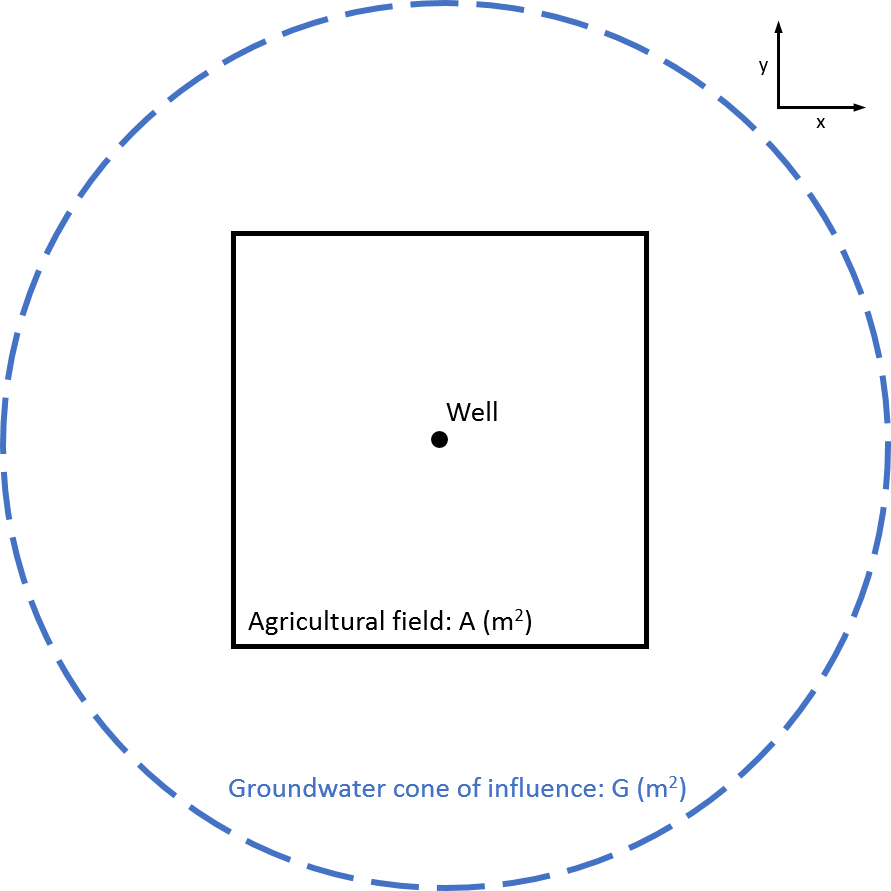
\includegraphics[width=0.4\linewidth]{Crop_cover}
 \captionsetup{justification=centering}
 \caption{Fictive schematic of crop cover area (C$_\%$)}
 \label{fig:Crop_cover}
\end{figure}

The A over G ratio ($C_{\%}$) shows top-view perspectives of spatially concatenated multiplication of agricultural fields, as visualized in Figure (\ref{fig:Crop_cover}). High $C_{\%}$ values (close to one) suggest the implementation of agricultural fields is possible at close mutual distance. \\

\begin{equation}
 C_{\%} = \frac{A}{G}
\label{eq:RR}
\end{equation}

Where  C$_{\%}$ is the crop cover ratio (-), $A$ (m$^2$) is the crop specific agricultural field size and $G$ (m$^2$) is the areal groundwater cone of influence. \\

\textbf{Financial yield} \\
Based on the known agricultural field size and (average) agricultural yield (unshelled groundnut 1.25 ton/ha) yield expression in weight is possible. Moreover weighted crop prices are also known. Because of this the first known water withdrawal volumes can be expressed in financial returns. From consistence considerations it is chosen to express the financial returns in US dollars. As a last step the The July 7$th$ Bloomberg financial exchange rate is applied: 0.2081 USD/GHS \citep{Bloomberg2018}. \\

\subsection{Water withdrawal: costs}
Profits are accompanied by costs. For this research all Capital Expenditures(CAPEX) are unknown and ignored. The same applies for large parts of the Operating Expenses (OPEX), e.g. farmer wage and fertilizer costs. The only costs accounted are related to the energy (diesel) consumption. Outcomes therefore purely focusses on the daily system usability. An impression is generated, whether or not regular ASR-system operation on its own is profitable. \\

\textbf{Energy Consumption} \\
First of all the available groundwater has to be lifted to the surface. Depends on the desired discharge, the lifting action requires a certain magnitude of power (Equation \ref{N_net}). Volumes of withdrawal (4 hours daily, 243 days) are known from the model simulation in the previous study section. For water displacement the difference between pump position and surface level (30m) is retained. An extra lift of 5 m is added to account for friction losses and the higher position (above surface) of the poly tank(s). A total head lift of 35 m is applied.

\begin{equation}
N_{net} =  g * Q * \Delta H
\label{N_net}
\end{equation}

Where $N_{net}$ (kW) is the net power required, g (m/s$^2$) is the gravitational acceleration (9.81 m/s$^2$), Q (m$^3$/s) is the discharge (total extracted volume of water over the yearly sum of pumping time (in seconds)) and $\Delta$H (m) is the net head (total lift) required. In this equation it is assumed the water has a density of 1000 kg/m$^3$.

In general, the use of power gets accompanied by losses (for example due to friction and turbulence). Ever single power-related equipment works at a certain level of efficiency. The power generator applied in fieldwork (Appendix \ref{chapter:fieldwork_set-up}) is used before. Because of datedness a generator efficiency of 70\% is estimated. The efficiency of the Pedrollo pump is dependent on discharge rate and/or head lift. An overview of the efficiency curve is present in Appendix \ref{chapter:Pedrollo_product_specs}. In this study it is assumed the pump can work on maximum efficiency (58\%) all time. Besides equipment losses, energy get lost due to mutual transmission. An extra efficiency value of 90\% is accounted \citep{VandeGiesen2013}. Result is a total (constant) ASR-system efficiency of 36.5 (\%).

\begin{equation}
 \eta_{total} =   \eta_{generator} * \eta_{transmission} * \eta_{pump} \end{equation}

Where $\eta_{total}$ (-) is the overall power efficiency, $\eta_{generator}$ (-) is the generator power efficiency, $\eta_{transmission}$ (-) is the transmission power efficiency and $\eta_{pump}$ (-) is the pump power efficiency. \\

The combination of total ASR-system efficiency and net required power provides the gross power required. It is this power what should be delivered by the generator to gain the desired volumes of water at the agricultural fields. Multiplying the gross power required by the total hours of pump oration returns the total energy consumption (kWh).

\begin{equation}
 N_{gross} =   \frac{N_{net}}{\eta_{total}}
\end{equation}

Where $N_{gross}$ (kW) is the gross power required, $N_{net}$ (kW) is the net power required and $\eta_{total}$ (-) is the overall power efficiency. \\

\textbf{Energy costs} \\
The Kipor power generator (Appendix \ref{chapter:fieldwork_set-up}) contains a 15 litre diesel tank. On a full tank the generator can operate for 6.5 hours. A fuel consumption of 2.31 l/h is taken into account. During operation the generator delivers a continuous power capacity of 4.5 kW \citep{TS242018}. Ghana diesel price of 5.03 GHS/l (begin of July) is adopted as normative \citep{GlobalPetrolPrices2018}. To make a good comparison with the agricultural yield, the Bloomberg financial exchange rate (0.2081 USD/GHS) is also applied on the fuel costs \citep{Bloomberg2018}.

\begin{equation}
 Cost_{fuel} =  \frac{consumption_{generator} * price_{fuel} * rate_{exchange}}{power_{generator}}
\end{equation}

Where $Cost_{fuel}$ (USD/kWh) is the price of fuel,  $consumption_{generator}$ (l/h) is the generator fuel consumption,  $price_{fuel}$ (GHS/l) is the fuel price in Ghana, $rate_{exchange}$ (USD/GHS) is the Bloomberg financial currency rate and $power_{generator}$ (kW) is the generator continuous power capacity. 

\section{Data processing (from water volumes to yield)}
\label{section:Data_processing}

\subsection{Crop cover area}

In Figure \ref{fig:Results_crop_cover_up_diam} an example of outcome. More to follow after first round of feedback graduation committee.

\begin{figure}[h!]
 \centering
 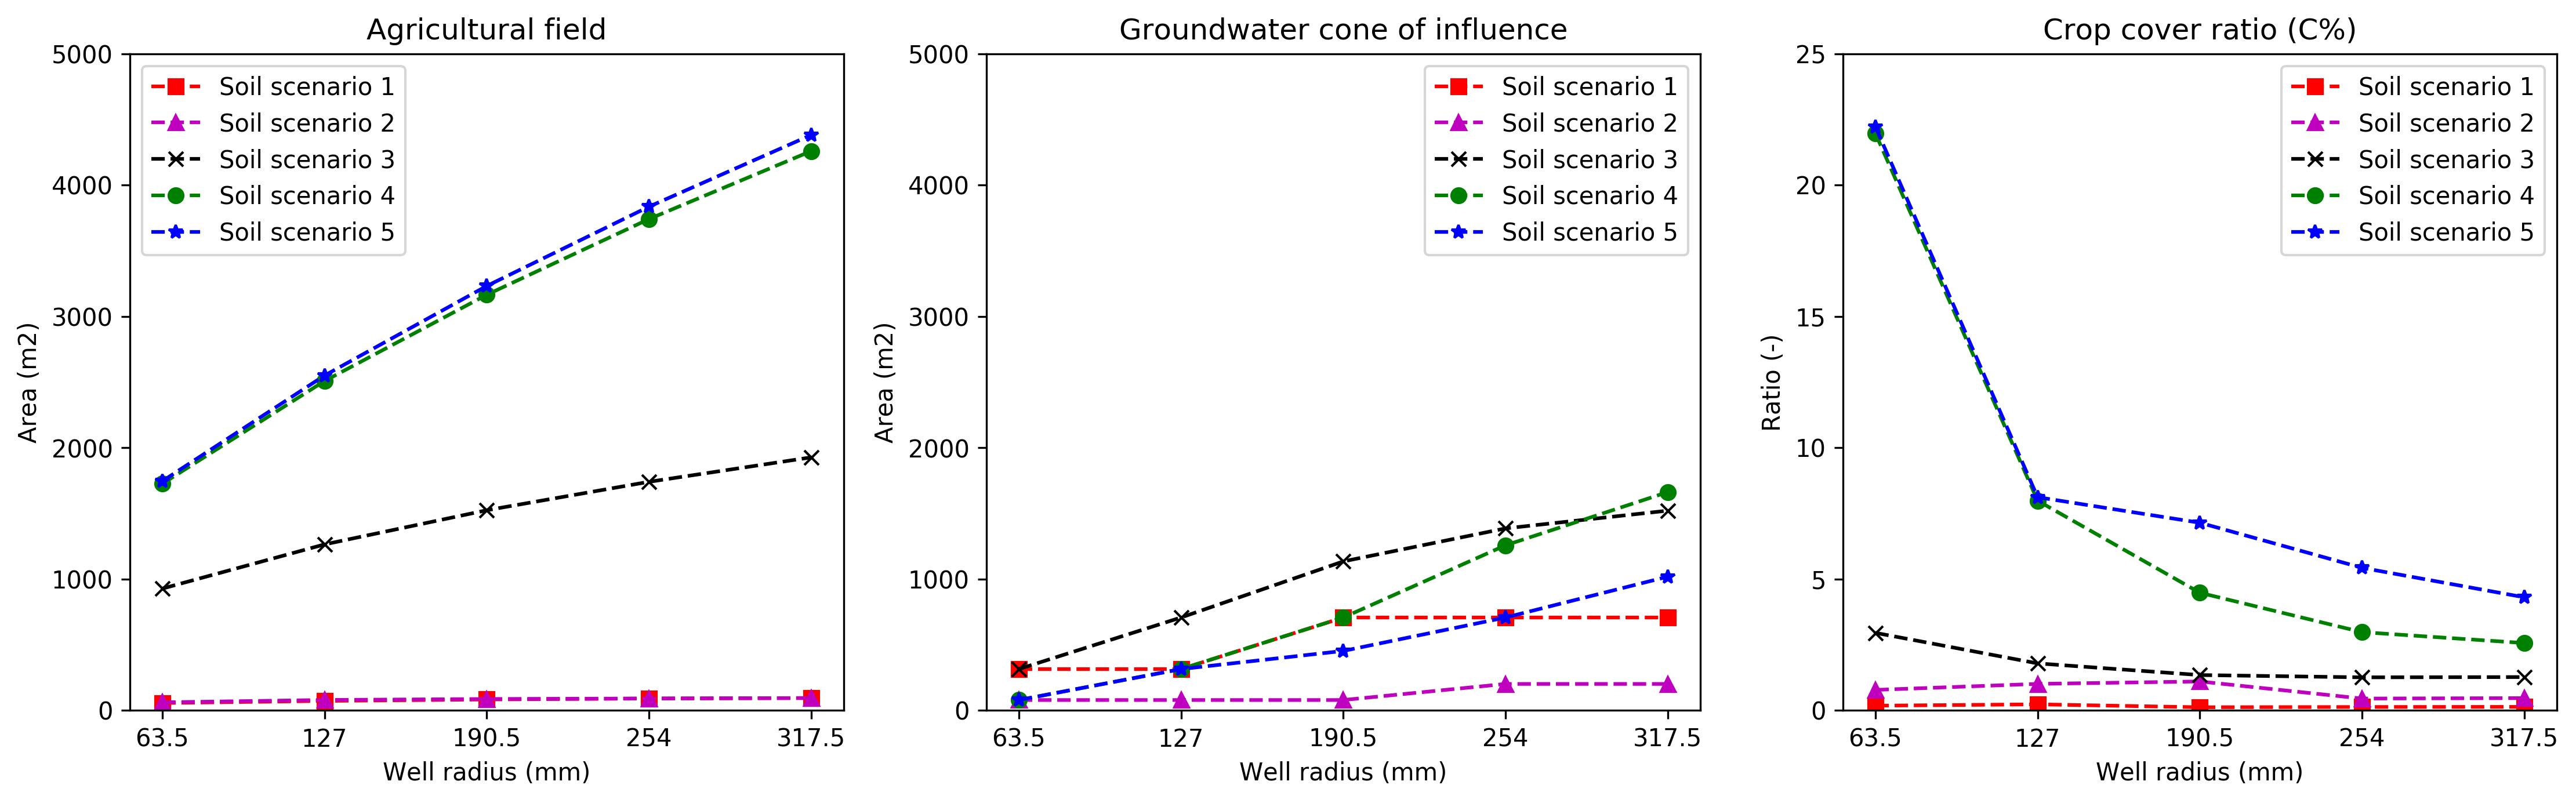
\includegraphics[width=1.0\linewidth]{Results_crop_cover_up_diam}
 \captionsetup{justification=centering} 
 \caption{Well diameter upscaling dependent results on net agricultural field size, areal groundwater cone of interest and "crop cover ratio"}
 \label{fig:Results_crop_cover_up_diam}
\end{figure}

\subsection{Financial yield}
In Figure \ref{fig:Results_financial_up_diam} an example of outcome. More to follow after first round of feedback graduation committee. 

\begin{figure}[h!]
 \centering
 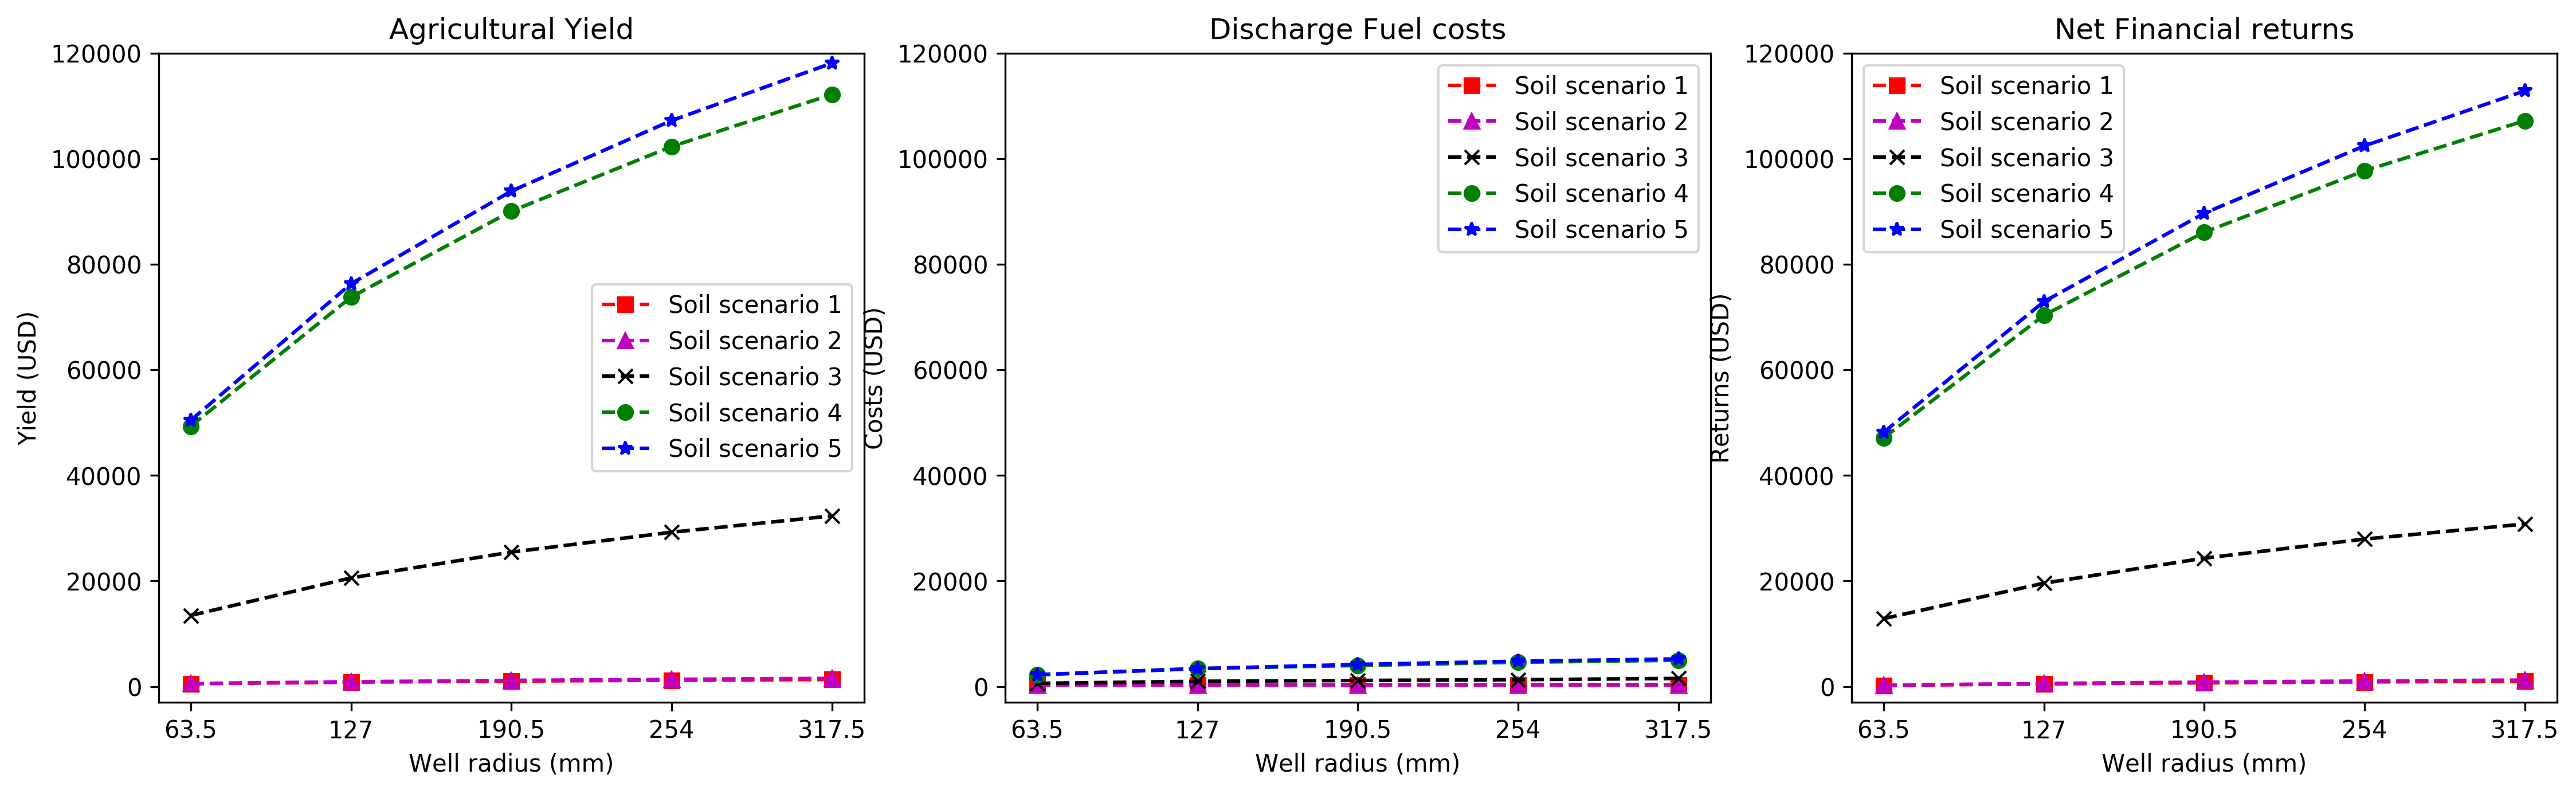
\includegraphics[width=1.0\linewidth]{Results_financial_up_diam}
 \captionsetup{justification=centering} 
 \caption{Well diameter upscaling dependent results on net agricultural yield, costs and net returns}
 \label{fig:Results_financial_up_diam}
\end{figure}

\section{Results \& conclusions}
\label{section:Yields_conclusions}

The preference to receive feedback before conclusions on this part are drawn. Moreover conclusions can and will be drawn after: 
\begin{itemize}
\item{1.} proper definition for head bound cone of influence 
\item{2.} pump-efficiency construction dependent on discharge 
\item{3.} optionally: the same can also be applied on different types of upscaling (time and cleaning). Added value: for example interesting to see what happens with fuel costs due to time increase
\item{4.} optionally: agricultural yields dependent on field-size 
\item{5.} optionally: take more OPEX or even CAPEX into account 
\end{itemize}